\chapter{Preliminaries}
\section{Motivation}\label{sec:motivation}

Natural language processing is a prominent component of artificial intelligence; since it allows the development of systems that have the ability to understand and generate human language, which facilitates communication between humans and computers, allowing \cite{torfi2020natural}. This is why currently many companies have become interested in its applications, such as task automation, customer experience improvement, automatic product recommendation, etc. Because of this the global natural language processing market size was valued at USD 27.73 billion in 2022 and is expected to expand at a compound annual growth rate (CAGR) of 40.4\% from 2023 to 2030 \cite{natural_language_processing_market_growth_report_2030_2030}. 

In particular, Question Answering systems in information retrieval are tasks that automatically answer the questions asked by humans in natural language using either a pre-structured database or a collection of natural language documents (\cite{7583963}). In other words, QA systems enable asking questions and retrieving answers using natural language queries (\cite{CAO2010962}). consider QA systems an advanced form of information retrieval. The demand for this kind of system increases on a daily basis since it delivers short, precise and question-specific answers (\cite{7755228}).

With the efforts from academic research, the QA subject has attracts growing interest around the world and the main evidence of this is the IBM Watson (\cite{6177724}). Some key advancements and applications in the field of automatic question answering include:

\begin{itemize}
    \item Personalized product recommendation models for automated question-answering robots using deep learning, which has shown better performance in terms of training loss and recommendation accuracy compared to other models (\cite{Peng2022}).

    \item A large number of machine reading comprehension models based on deep learning, which have been developed to improve the performance of automatic question answering systems (\cite{9072442}).
\newpage
    \item A chatbot analytics system based on question answering and deep learning, which has been built to answer questions about movies from movie reviews using a sequence-to-sequence (Seq2Seq) word embedding model (\cite{shah2020chatbot}).

    \item A question-answer pair generation system using deep learning, which aims to save time and reduce effort in various fields such as school assignments, law practicing, and self-assessments (\cite{9544654}).

    \item Large Language Models like GPT, LlaMA and Bard have revolutionized the NLP field, showing improved performance in many tasks including question answering (\cite{hadi2023large}). 
 
\end{itemize}



\begin{figure}[h!]
    \centering%width=0.7\linewidth
    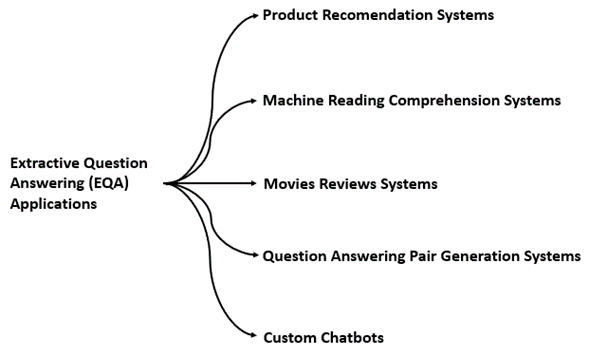
\includegraphics[width=\linewidth]{Figures/Preliminares/applications.png}
    \caption{Extractive Question Answering Applications}
    \label{fig:summary_apps}
\end{figure}


Recurrent neural networks and closed recurrent neural networks have been established as effective approaches for natural language processing tasks, including the EQA task. However, recurrent models process element by element of a sequence, which makes them non-parallelizable and does not allow them to calculate long-term relationships in sequences of texts. Attention mechanisms appeared to solve these problems, with transformer architecture being the first architecture to be based entirely on attention mechanisms \cite{pearce2021comparative}. Large pre-trained language models such as BERT \cite{devlin2018bert}, Roberta \cite{liu2019roberta}, and Distilbert \cite{sanh2019distilbert} use encoder-only transformer architectures for the EQA task; because this task is merely extractive. 


However, despite remarkable performances on answer prediction, these approaches are black-box by nature, lacking of the capability of providing explanations for their predictions (\cite{thayaparan2020explanationlp}). It is in this context that the interpretability of deep learning models plays a pivotal role.

Understanding the inner workings of these models is not only an intellectual pursuit but a necessity for practical deployment. Interpretability is the key to demystifying the decision-making processes of deep learning models, providing insights into why a particular answer is generated (\cite{dao2020demystifying}). This interpretative lens is vital for building robust and trustworthy systems, ensuring accountability, and facilitating human-AI collaboration (\cite{caldwell2022agile}.

\begin{figure}[h!]
    \centering%width=0.7\linewidth
    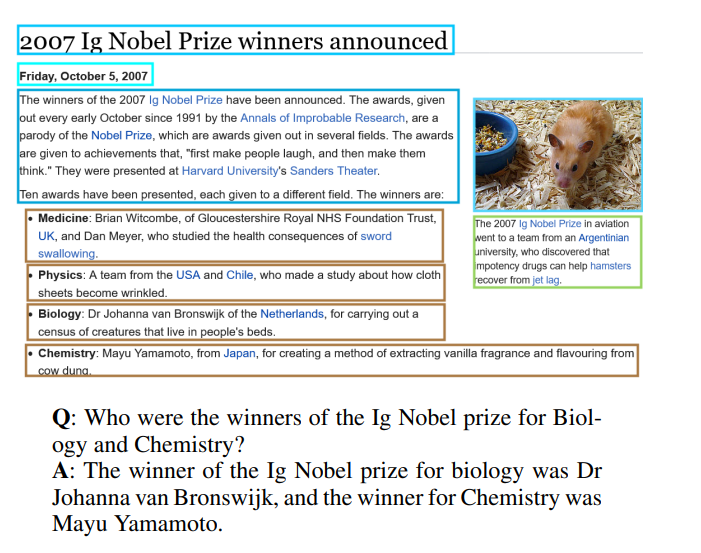
\includegraphics[width=\linewidth]{Figures/Preliminares/visualmrc_example.png}
    \caption{Scheme of an EQA task applied in the context of web pages, which highlights the need to understand in which regions of the image the most relevant text is located when answering a question to a user.}
    \label{fig:example_vmrc}
\end{figure}

\newpage

The Control and Digital Signal Processing Group (GCPDS) of the National University of Colombia is immersed in the research and development of technologies that promote efficiency and accessibility in the interaction between the university community and institutional information. In this context, the interest in working on question-answer systems is based on our vision of optimizing access to key documents, such as regulations, resolutions and minutes, within the university environment. Currently, we are in the process of building a chatbot that will allow any member of the community to get accurate and quick answers to their questions about university documentation. The main objective of this initiative is to facilitate access to information, reduce response times by administrative staff and maximize the use of the latter's time for tasks with greater added value.

In conclusion, the intersection of automatic question answering tasks and the interpretability of deep learning models represents a critical juncture in the evolution of intelligent systems. As these models advance in their ability to provide accurate responses to user queries, the need for interpretability becomes increasingly pronounced. In the context of web page information extraction for question answering, interpretability measures play a pivotal role. By dissecting the decision-making processes of the deep learning model, we gain the ability to identify the specific elements within web pages that contribute most significantly to the generated answers. This not only enhances user trust by offering transparency in the system's reasoning but also provides actionable insights for developers to optimize web page structures. The practical use case outlined here underscores the tangible impact of interpretability measures, serving as a catalyst for the development of more reliable, transparent, and user-centric deep learning-based question answering systems. As we navigate the frontier of AI applications, the symbiotic relationship between interpretability and task performance becomes indispensable, paving the way for responsible and trustworthy artificial intelligence.

